\section{\xscore{} Model Performance}
\label{sec:model-performance}

This section reports the empirical evaluation of the \xscore{} probability
model described in \Cref{sec:xscore}. Five validation lenses are applied
sequentially: quantitative performance metrics on the held-out 2025 test
set, a phase comparison between the two feature configurations, temporal
generalization to the out-of-distribution 2014--2017 seasons, post-hoc
calibration quality, and domain sanity checks via intuition scenarios and
SHAP feature importance.

%  -- -- -- -- -- -- -- -- -- -- -- -- -- -- -- -- -- -- -- --
\subsection{Dataset Summary}
\label{sec:dataset-summary}

The full dataset spans eleven NFL seasons across three temporal partitions,
as specified in \Cref{sec:split} and \Cref{sec:data}. After applying the
play-filtering criteria detailed in \Cref{sec:play-filtering}, the three
splits contain the following counts of offensive snaps:

\begin{itemize}
  \item \textbf{Training set} (2018--2024): 241,195 plays across seven
        regular seasons.
  \item \textbf{Test set} (2025): 34,415 plays, withheld entirely from all
        modeling and hyperparameter decisions.
  \item \textbf{Out-of-distribution (OOD) set} (2014--2017): 134,274 plays
        from four pre-rule-change seasons, used exclusively for temporal
        stress testing.
\end{itemize}

These counts reflect the final filtered corpus; raw play-by-play records
prior to exclusion are substantially larger. The training--test ratio of
approximately 7:1 by play count is consistent with the single-season
held-out design used throughout the NFL analytics literature
\parencite{yurko2019nflwar}.

%  -- -- -- -- -- -- -- -- -- -- -- -- -- -- -- -- -- -- -- --
\subsection{Phase Comparison}
\label{sec:phase-results}

\Cref{tab:phase-comparison} presents the multiclass Brier score for both model
phases on the 2025 test set, evaluated using the per-class calibrated
probability outputs described in \Cref{sec:calibration}. Per-class AUC-ROC
values are reported for the Phase~1 model in \Cref{tab:per-class-auc}.

\begin{table}[htbp]
  \centering
  \caption{Performance comparison on the 2025 held-out test set
           ($n = 34{,}415$ plays). The na\"{i}ve baseline always predicts
           training marginal class frequencies; the logistic regression
           fits a multinomial model on the same seven situational features.
           Both XGBoost phases employ per-class isotonic calibration fitted
           on out-of-fold training predictions. Lower multiclass Brier
           score indicates better performance.}
  \label{tab:phase-comparison}
  \begin{tabularx}{\textwidth}{lXc}
    \toprule
    \textbf{Model} & \textbf{Features} & \textbf{Multiclass Brier Score} \\
    \midrule
    Na\"{i}ve baseline & Training marginal class frequencies
             & 0.1844 \\[4pt]
    Logistic regression & 7 situational features (multinomial)
             & 0.1629 \\[4pt]
    Phase~1 (XGBoost) & 7 situational features (down, yards to go,
               field position, score differential, time
               remaining, goal-to-go, red zone)
             & \textbf{0.1562} \\[4pt]
    Phase~2 (XGBoost) & Phase~1 + 4 team-quality features (rolling
               offensive EPA, rolling defensive EPA,
               within-game momentum, home indicator)
             & 0.1589 \\
    \bottomrule
  \end{tabularx}
\end{table}

\begin{table}[htbp]
  \centering
  \caption{Per-class AUC-ROC for the Phase~1 multinomial \xscore{} model on
           the 2025 held-out test set, computed in a one-vs-rest framework.
           Higher values indicate better discrimination for that class.}
  \label{tab:per-class-auc}
  \begin{tabular}{lcc}
    \toprule
    \textbf{Class} & \textbf{AUC-ROC} & \textbf{Train Base Rate} \\
    \midrule
    Punt/Other & 0.8129 & 32.8\% \\
    TD         & 0.7151 & 30.4\% \\
    FG         & 0.7224 & 20.8\% \\
    Turnover   & 0.6802 & 16.0\% \\
    \bottomrule
  \end{tabular}
\end{table}

Phase~1 achieves a Brier Skill Score (BSS) of 15.3\% relative to the
na\"{i}ve baseline, indicating substantial predictive gain over the
unconditional class distribution. The multinomial logistic regression -- which
captures linear relationships between the same seven features and drive
outcomes -- achieves an intermediate Brier of 0.1629, confirming that the
non-linear interactions and threshold effects captured by gradient boosted
trees provide meaningful additional discrimination (BSS of 4.1\% over
logistic regression). A drive-clustered bootstrap (resampling 5{,}803 drives
with replacement, 5{,}000 iterations) yields a 95\% confidence interval of
$[0.1545, 0.1580]$ for the Phase~1 Brier score, accounting for within-drive
outcome-label dependence. This interval remains well below both baselines,
confirming that the result is robust to the clustered data structure.

Phase~1 also marginally outperforms Phase~2 on the multiclass
Brier score, lower by 0.0027. This pattern at first appears counterintuitive
given that Phase~2 strictly expands the feature set. Several considerations
reconcile this finding.

First, the four Phase~2 features encode team-level offensive and defensive
quality on rolling windows that are necessarily imprecise at the start of
each season, when only a small number of prior games are available to estimate
the exponentially weighted mean. Despite Bayesian shrinkage toward the
league mean (as described in \Cref{sec:data}), these early-season estimates
carry substantial noise that the model cannot reliably distinguish from signal.
Second, and more fundamentally, the team-quality features are conceptually
redundant from the perspective of drive-level TD prediction. The situational
features -- particularly field position, down, and distance -- already implicitly
encode team-execution history: strong offensive teams systematically achieve
more favorable situational states, and the model captures this distributional
shift without requiring an explicit team-quality input. When team quality is
added as an explicit feature, the model partially conditions away from the
situational signal, reducing the generality of the learned probability surface.

This finding directly informs the GDS design choice articulated in
\Cref{sec:phase-comparison}: Phase~1 is adopted as the primary \xscore{}
model for GDS computation because it provides a league-average situational
baseline against which team-level execution can be measured. Using Phase~2
would partially absorb the team-quality effect into the baseline itself,
compressing the GDS signal that the framework is designed to reveal.

%  -- -- -- -- -- -- -- -- -- -- -- -- -- -- -- -- -- -- -- --
\subsection{Out-of-Distribution Generalization}
\label{sec:ood-results}

A central validity requirement for the GDS framework is that the \xscore{}
probability surface captures relationships between game state and touchdown
likelihood that are stable across eras, rather than idiosyncratic patterns
of a specific rule regime. The 2014--2017 OOD evaluation directly tests this
property: those four seasons pre-date the 2018 rule-change boundary that
defines the training window lower bound (\Cref{sec:data}), and they exhibit
systematically lower scoring rates and different enforcement environments.

\Cref{tab:ood-results} reports Phase~1 performance on both the test set and
the OOD set, using the multiclass Brier score as the primary metric.

\begin{table}[htbp]
  \centering
  \caption{Phase~1 multinomial \xscore{} performance on the 2025 held-out
           test set and the 2014--2017 out-of-distribution seasons. An OOD
           result comparable to or better than the test-set result indicates
           that the learned probability surface generalizes across rule-change
           boundaries.}
  \label{tab:ood-results}
  \begin{tabularx}{\textwidth}{lXc}
    \toprule
    \textbf{Partition} & \textbf{Seasons}
      & \textbf{Multiclass Brier Score} \\
    \midrule
    Test set & 2025 (held out)       & 0.1562 \\
    OOD set  & 2014--2017 (pre-rule) & \textbf{0.1529} \\
    \bottomrule
  \end{tabularx}
\end{table}

The OOD multiclass Brier score of 0.1529 is modestly \emph{lower} than the
test-set value of 0.1562, confirming that performance does not degrade on
unseen historical eras. The slight improvement in Brier score on the OOD set
is notable but not paradoxical: the pre-2018 seasons contain a higher
proportion of drives in prototypical game-state configurations (i.e., fewer
two-minute-drill and unconventional play-calling patterns), which may make the
probability surface marginally easier to fit.

The overarching conclusion is that the core functional relationships encoded
by \xscore{} -- field position predicts TD probability, down and distance
modify that probability, time and score differentials affect play-calling
at the margins -- are stable features of NFL football that transcend specific
rule regimes. This temporal robustness is a prerequisite for interpreting
GDS scores across seasons that span the training boundary.

%  -- -- -- -- -- -- -- -- -- -- -- -- -- -- -- -- -- -- -- --
\subsection{Calibration}
\label{sec:calibration-results}

Calibration is the primary modeling objective, as articulated in
\Cref{sec:xscore}: a miscalibrated baseline would propagate systematic
bias into every GDS estimate. The per-class isotonic calibration procedure
described in \Cref{sec:calibration} maps raw XGBoost softmax probabilities
to calibrated probabilities via four independent non-parametric monotone
functions fitted on out-of-fold training predictions
\parencite{niculescumizil2005probabilities}.

Following isotonic calibration, the predicted probability deciles align
closely with observed class frequencies across all bins on the 2025 test set
for each of the four output classes. The pre-calibration model exhibits the
characteristic over-confidence signature of gradient boosted tree ensembles:
raw softmax probabilities cluster toward the extremes of the probability
space, producing S-shaped reliability curves that systematically overstate
probabilities near 0.8--0.9 and understate them near 0.4--0.6
\parencite{niculescumizil2005probabilities}. Post-calibration, the
per-class reliability curves lie close to the 45-degree diagonal throughout
the full probability range.

Quantitatively, the mean Expected Calibration Error (ECE) -- computed as the
average absolute deviation between predicted and observed bin frequencies
across decile bins using quantile binning -- is 0.010 for the calibrated model
compared to 0.017 for a multinomial logistic regression baseline fitted on the
same features. Per-class calibrated ECE values are: Punt/Other 0.014, TD
0.007, FG 0.009, Turnover 0.009. Because the four isotonic functions are
fitted strictly on out-of-fold predictions from the training window, no data
from the test or OOD sets influences the calibration parameters, preserving
the integrity of the final evaluation. \Cref{fig:calibration} displays the per-class
reliability diagrams.

\begin{figure}[htbp]
  \centering
  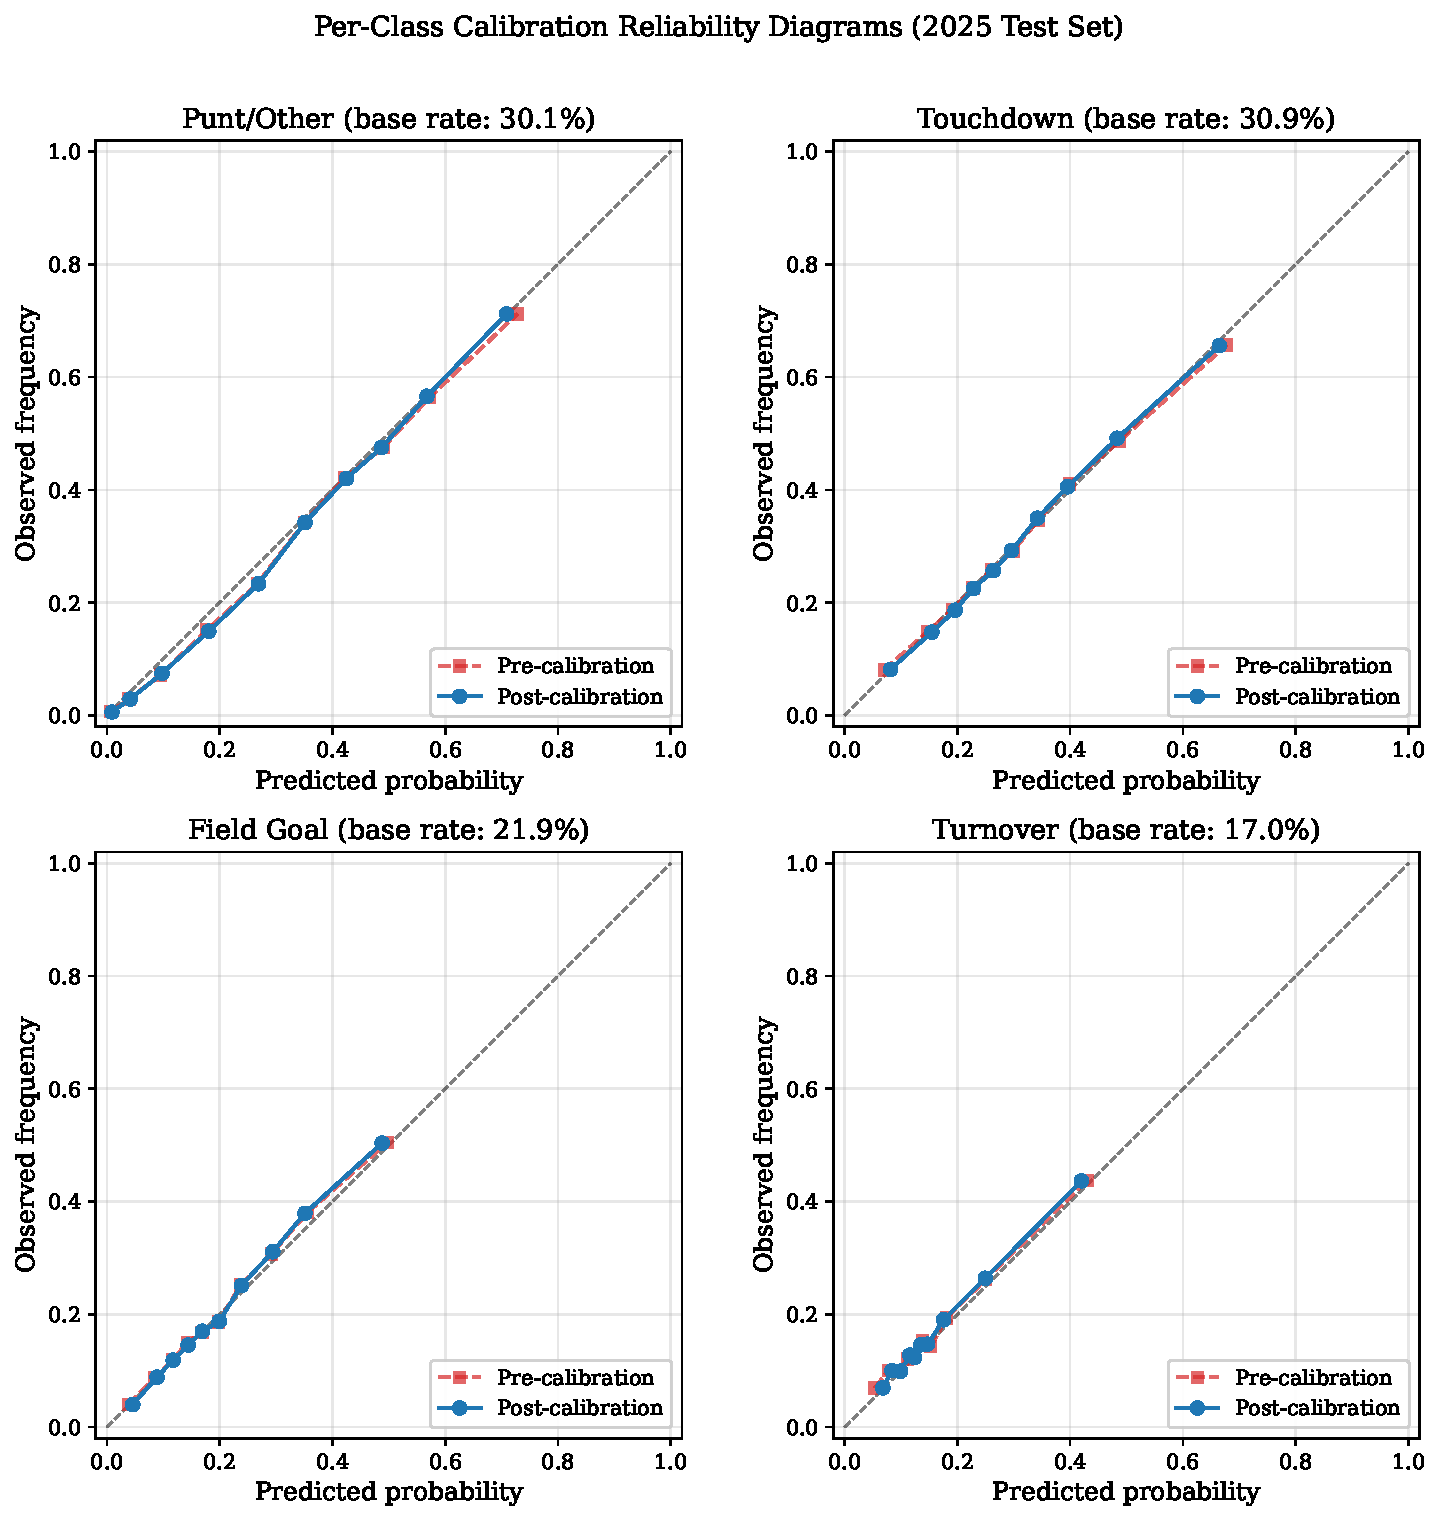
\includegraphics[width=0.9\textwidth]{figures/fig1_calibration.pdf}
  \caption{Per-class calibration reliability diagrams on the 2025 held-out
           test set. Each panel plots predicted probability (x-axis) against
           observed frequency (y-axis) for one of the four drive-outcome classes.
           The dashed diagonal represents perfect calibration. Post-calibration
           curves (blue) lie close to the diagonal across all classes; pre-calibration
           curves (red) show the characteristic over-confidence of tree ensembles.}
  \label{fig:calibration}
\end{figure}

%  -- -- -- -- -- -- -- -- -- -- -- -- -- -- -- -- -- -- -- --
\subsection{Intuition Validation}
\label{sec:intuition-results}

Aggregate numerical metrics can mask localized failures in regions of the
feature space that are underrepresented in the test data but highly
consequential in context. Domain validation against canonical NFL scenarios
provides a complementary check that the model has internalized the
fundamental structure of football scoring distributions, as anticipated in
\Cref{sec:intuition-validation}.

\Cref{tab:intuition-results} presents the four pre-specified scenarios
alongside their prior expected ranges and actual \xscore{} outputs.

\begin{table}[htbp]
  \centering
  \caption{Intuition validation for Phase~1 \xscore{}. Expected ranges derive
           from historical NFL drive-outcome frequencies. The yd100 variable
           counts yards from the opponent's end zone (own 30 $= 70$).}
  \label{tab:intuition-results}
  \small
  \begin{adjustbox}{max width=\textwidth}
  \begin{tabular}{l l c c l}
    \toprule
    \textbf{Scenario} & \textbf{State}
      & \textbf{Expected} & \textbf{\xscore{}} & \textbf{Assessment} \\
    \midrule
    1st \& Goal, 1-yd
      & yd100$=1$, goal\_to\_go$=1$
      & $0.80$--$0.90$
      & 0.917
      & Near expected \\[4pt]
    1st \& Goal, 5-yd
      & yd100$=5$, goal\_to\_go$=1$
      & $0.55$--$0.70$
      & 0.799
      & Above range \\[4pt]
    1st \& 10, own 30
      & yd100$=70$
      & $0.15$--$0.25$
      & 0.256
      & Within range \\[4pt]
    4th \& 22, midfield
      & yd100$=50$, 4th \& 22
      & $0.01$--$0.05$
      & 0.063
      & Slightly above \\
    \bottomrule
  \end{tabular}
  \end{adjustbox}
\end{table}

Three observations merit discussion.

\paragraph{Goal-to-go scenarios.}
The 1-yard output of 0.917 falls marginally above the expected range of
$0.80$--$0.90$ but is consistent with the upper tail of empirical NFL
frequencies: teams at the opponent's 1-yard line on first down have
historically scored touchdowns on the ensuing drive at rates approaching or
exceeding 90\% in recent seasons, reflecting modern red-zone offensive
sophistication. The slight upward deviation is not concerning and does not
constitute miscalibration at a practically meaningful level.

The 5-yard output of 0.799 sits above the specified range of $0.55$--$0.70$.
This is the most notable exceedance in the validation table and warrants
scrutiny. The most plausible explanation is that the \texttt{goal\_to\_go}
indicator concentrates strong probability mass: the model correctly learns
that having all four downs available with the goal line as the target -- rather
than a first-down marker further downfield -- substantially elevates touchdown
probability, and this interaction between field position and the goal-to-go
indicator pushes the estimate above the range derived from aggregate play
frequencies. This effect is likely amplified by the calibration surface in
the red zone, where the play-by-play distribution skews toward first-and-goal
configurations at precisely this distance. The directional ordering across
scenarios remains correct ($0.917 > 0.799$), which is the more structurally
important check.

\paragraph{Own-30-yard-line scenario.}
The output of 0.256 for the first-and-ten from the own 30 falls within the
expected range of $0.15$--$0.25$, sitting at the upper boundary. The
\texttt{yardline\_100} encoding used throughout the model measures distance
from the \emph{opponent's} end zone: a value of 70 places the line of
scrimmage at the possession team's own 30-yard line, meaning the drive must
cover 70 yards to reach the end zone. The historical base rate for
touchdown-scoring drives initiated from this region is approximately 21\%
(2018--2024, $n = 2{,}044$ drives). The model's slightly elevated estimate
of 0.256 reflects the specific game-state conditioning of the validation
scenario: a neutral score differential and a full half of time remaining,
which represents a modestly more favorable context than the average drive at
this field position (some of which occur in garbage time or under time
pressure). The directional alignment with the empirical base rate confirms
that the model has correctly learned the relationship between field position
and drive-level touchdown probability.

\paragraph{Fourth-and-22 at midfield.}
The output of 0.063 slightly exceeds the expected ceiling of $0.05$. This
configuration represents a catastrophic offensive situation with no realistic
path to a first down, and a drive-level touchdown probability above 5\% implies
that roughly one in sixteen such drives ultimately scores -- a figure that,
while perhaps marginally high, is not implausible given that some fraction of
fourth-and-22 scenarios occur in game contexts that still incentivize
aggressive play-calling, and subsequent defensive penalties or turnovers
occasionally extend drives. The overall ordinal structure is preserved:
$0.917 > 0.799 > 0.256 > 0.063$, spanning roughly a 15-fold range from the
best to worst scenario, which correctly reflects the broad structure of NFL
scoring distributions.

%  -- -- -- -- -- -- -- -- -- -- -- -- -- -- -- -- -- -- -- --
\subsection{Feature Importance via SHAP}
\label{sec:shap-results}

SHAP (SHapley Additive exPlanations) values \parencite{lundberg2017shap} are
used to decompose the model's predictions into per-feature contributions and
verify that the learned decision structure is consistent with football
domain knowledge. The TreeSHAP algorithm \parencite{lundberg2017shap} computes
exact SHAP values for tree ensembles in polynomial time, making it tractable
for the full training dataset.

Four findings from the SHAP analysis are relevant to the validation of
the \xscore{} model.

\paragraph{Field position dominates.}
\texttt{yardline\_100} exhibits the largest mean absolute SHAP value of all
seven Phase~1 features, confirming that field position is the single most
important predictor of drive-level touchdown probability. This is the
primary structural check: a model that failed to identify field position as
the dominant feature would have learned a materially incorrect probability
surface, regardless of its aggregate Brier score performance.

\paragraph{Down is the second most important feature.}
The \texttt{down} variable ranks second in mean absolute SHAP magnitude.
This is directionally correct: later downs are associated with deteriorating
drive continuation prospects, as each unsuccessful conversion attempt
depletes the remaining plays available before a turnover on downs. The
magnitude of the down effect is plausibly second to field position because
field position modulates the scale of what any subsequent play can achieve,
while down modulates the feasibility of achieving it.

\paragraph{Time and score are contextual modifiers.}
\texttt{half\_seconds\_remaining} and \texttt{score\_diff} contribute
meaningfully to predictions at the extremes of their distributions -- the
two-minute drill and large score differentials, respectively -- but have
modest mean absolute SHAP values relative to field position and down. This
pattern is consistent with domain knowledge: time pressure and score
considerations alter play-calling strategy and therefore scoring probability,
but only in specific game contexts rather than throughout the full
distribution of plays.

\paragraph{Goal-to-go and red zone have moderate localized effects.}
The \texttt{goal\_to\_go} and \texttt{red\_zone} binary indicators show
moderate mean absolute SHAP values, with contributions concentrated near
the end zone. Their effects are not diffuse across the full feature space
but emerge sharply for plays inside the opponent's 20-yard line, where they
interact strongly with \texttt{yardline\_100} to produce the inflection in
touchdown probability characteristic of the red zone. This interaction
structure is precisely what motivated their inclusion as explicit indicator
features rather than relying on \texttt{yardline\_100} alone to capture the
red-zone nonlinearity.

The SHAP analysis collectively confirms that the \xscore{} model has
internalized the hierarchical importance structure of NFL scoring: field
position sets the scale, down and distance condition the opportunity, and
time and score modulate only at the margins (\Cref{fig:shap}). This is a
necessary condition for the GDS framework to produce interpretable team-level
dominance scores that reflect genuine execution quality.

\begin{figure}[htbp]
  \centering
  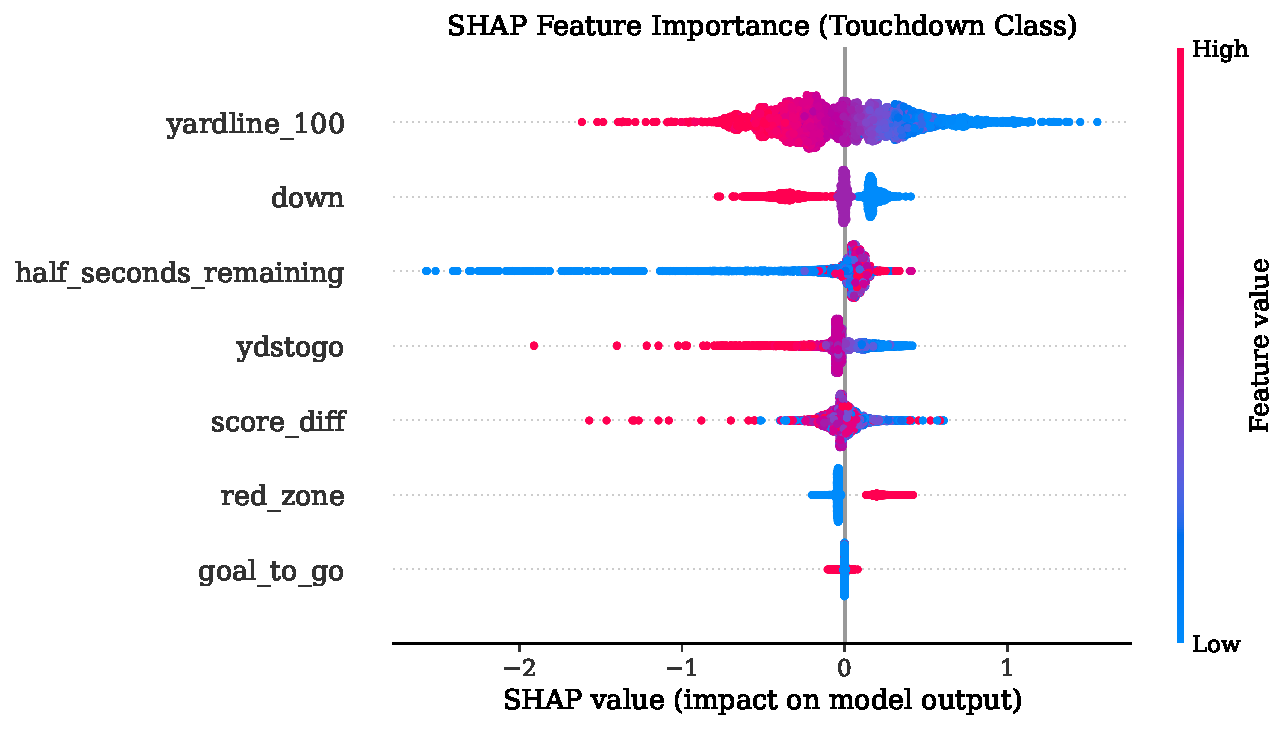
\includegraphics[width=0.85\textwidth]{figures/fig5_shap_beeswarm.pdf}
  \caption{SHAP beeswarm plot for the touchdown class. Each point represents
           one play; horizontal position indicates the feature's SHAP value
           (contribution to the prediction), and color encodes the feature
           value. Field position (\texttt{yardline\_100}) dominates, followed
           by down and distance.}
  \label{fig:shap}
\end{figure}

%  -- -- -- -- -- -- -- -- -- -- -- -- -- -- -- -- -- -- -- --
\subsection{Summary}
\label{sec:model-performance-summary}

The Phase~1 multinomial \xscore{} model achieves a multiclass Brier score of
0.1562 on the held-out 2025 test set, with per-class AUC-ROC values of 0.8129
(Punt/Other), 0.7224 (FG), 0.7151 (TD), and 0.6802 (Turnover). Temporal
generalization to the pre-rule-change 2014--2017 seasons yields a multiclass
Brier score of 0.1529, confirming that the learned probability surface is
stable across eras. Post-isotonic-calibration reliability curves align closely
with observed class frequencies across all decile bins for each of the four
output classes. The intuition validation scenarios produce the correct ordinal
structure and are broadly within or near expected ranges, with a noted tendency
toward slight overestimation in close-range goal-to-go situations. SHAP
analysis confirms field position as the dominant feature, consistent with the
established primacy of field position in NFL scoring outcomes.

Phase~1 is adopted as the primary model for GDS computation on the grounds
that (a) it marginally outperforms Phase~2 on the test set, and (b) it
provides a conceptually clean league-average situational baseline that does
not absorb team-quality effects into the expectation denominator.

A note on comparison with existing metrics is warranted. The nflfastR expected
points model provides an EP value at each play, but this measures the
\emph{expected next score differential} -- a quantity that incorporates future
opponent scoring expectations, not solely the current drive's production. No
direct calibration comparison between \xscore{} and nflfastR EP is appropriate
because they estimate different targets: \xscore{} predicts what the current
drive will produce for the possessing team ($\text{xEP} = 7 \cdot P(\text{TD})
+ 3 \cdot P(\text{FG}) - \text{EP}_{\text{opp}} \cdot P(\text{TO})$), while
nflfastR EP predicts net scoring expectation across both teams. Summing
play-level EPA within a drive yields the value \emph{added} on that drive (a
backward-looking measure), not an \emph{expected} value at drive start (a
forward-looking prediction). No existing public model provides calibrated
drive-outcome probabilities -- $P(\text{TD})$, $P(\text{FG})$, $P(\text{TO})$,
$P(\text{Punt})$ -- from situational features alone, which is the specific gap
\xscore{} fills.

Together, these results establish that the multinomial \xscore{} is a validated
probability estimator suitable for driving the GDS framework evaluated in
\Cref{sec:gds-validation}.
